\chapter{Introduction}
\label{chapter:introduction}

\graphicspath{{Chapter1/Figs/}{Chapter1/Figs/PDF/}{Chapter1/Figs/}}%

\subsection{Background}

\subsubsection{The normal cell}

  The human body comprises trillions of small units called cells. Cells are the building blocks of the human body, with the ability to grow, replicate and die. The center of eukaryotic cells is the nucleus. Functions of the nucleus are to store hereditary information in the chromosomes and to coordinate vital cell activities like growth, metabolism, protein synthesis, replication and death. The nucleus of a normal human cell contains two copies of each of the 22 autosomal chromosomes and 2 sex chromosomes. Chromosomes consist of tightly coiled double-helix shaped DNA, wrapped around histones. Strands of a DNA molecule are made up of four nucleotide bases: adenine (A), thymine (T), guanine (G) and cytosine (C). Functional units of the DNA molecule are called genes. Human cells contain about 25000 protein-coding genes. 

  Another molecule that plays a crucial role in the cells is RNA. This is a single-stranded molecule, containing nucleotide bases A, G, C and uracil(U) instead of T. Information stored in the DNA is transferred via these RNA molecules. The  process in which an RNA molecule is synthesized using DNA as a template, is called transcription. During transcription several types of coding and non-coding RNA molecules are expressed from DNA, all of them together forming the transcriptome. In this thesis besides DNA the following RNA molecules were further investigated:
\begin{itemize}
\item Messenger RNA (mRNA). These molecules convey the information stored in DNA outside the nucleus into the cytoplasm, where they are translated into proteins.
\item microRNA (miRNA). These molecules represent a major class of non-coding RNA molecules, meaning they are not translated into proteins. miRNAs are small (about 22 nucleotides in length) molecules that bind to mRNAs by (partial) complementarity thereby inhibiting translation of these mRNAs into proteins or inducing mRNA degradation/destabilization. miRNAs are becoming more and more recognized as major players in both normal cellular regulation and disease.
\end{itemize}

\subsubsection{(Epi)genetic alterations in the cell}

During cancer development, epigenetic and genetic abnormalities occur on the level of the genome resulting in an altered transcriptome. Accumulation of (epi)genetic alterations in cancer cells can result in permanent activation of oncogenes and inactivation of tumor suppressor genes. Oncogenes stimulate cell growth and prevent cell differentiation. Aberrant expression of oncogenes in tumor cells promote tumor formation. Tumor suppressor genes in the normal cell slow down cell division, repair DNA mistakes, initiate differentiation, and induce cell death if necessary. Aberrant silencing of tumor suppressor genes in cancer cells therefore also promotes tumor formation. 

Epigenetic changes alter gene expression without changing the DNA sequence. One of the best known mechanisms is DNA methylation. DNA methylation is the process where a methyl ($\textrm{CH}_3$) group is added to the cytosine within CpG dinucleotides. These CpG dinucleotides are enriched in specific regions of the genome, so-called CpG islands, which are often overlapping with promoter regions of genes. DNA hypermethylation of promoter regions alters accessibility of the DNA for transcription factors usually resulting in gene silencing. 

  Genetic abnormalities comprise changes to the DNA sequence, including mutations, structural and non-structural chromosomal aberrations. Mutations involve alterations in DNA sequence bases, which can lead to modification in the amount and structure of the resulting protein product, thereby influencing its function. Structural chromosomal aberrations appear as a rearrangement of parts of the genome usually without affecting the total amount of DNA. On the other hand, non-structural aberrations result in DNA copy number alterations where more than 2 copies (gain) or less than 2 copies (loss) are observed for specific parts of the genome. Abnormalities on the DNA level (genome) may be reflected on the RNA level, ultimately affecting protein synthesis. 

\subsubsection{Cervical cancer and the human papillomavirus (HPV)}

Cervical cancer is the fourth most commonly diagnosed cancer among females worldwide \cite{Ferlay2015}. The incidence of cervical cancer is highest in developing countries, where nearly $90\%$ of cervical cancer deaths occur, due to the absence of population based screening programs. Cervical cancer is caused by a persistent infection with high-risk types of the human papillomavirus (HPV) and develops via well-recognizable precancerous lesions. HPV is a double-stranded sexually transmitted DNA virus belonging to the Papillomaviridae family, which comprise more than 150 different types infecting either the skin or the mucosae lining the anogenital, respiratory and upper digestive tract. Among the mucosa-infecting HPV types, 15 are classified as high-risk types and are associated with cervical cancer. Together, HPV16 and HPV18 cause approximately $70\%$ of all cervical cancers. It is widely accepted that the involvement of high-risk types of HPV together with specific (epi)genetic modifications in the host cell genome, drive cervical carcinogenesis. 

\begin{figure}[h!]
\centering
\begin{tabular}{cc}
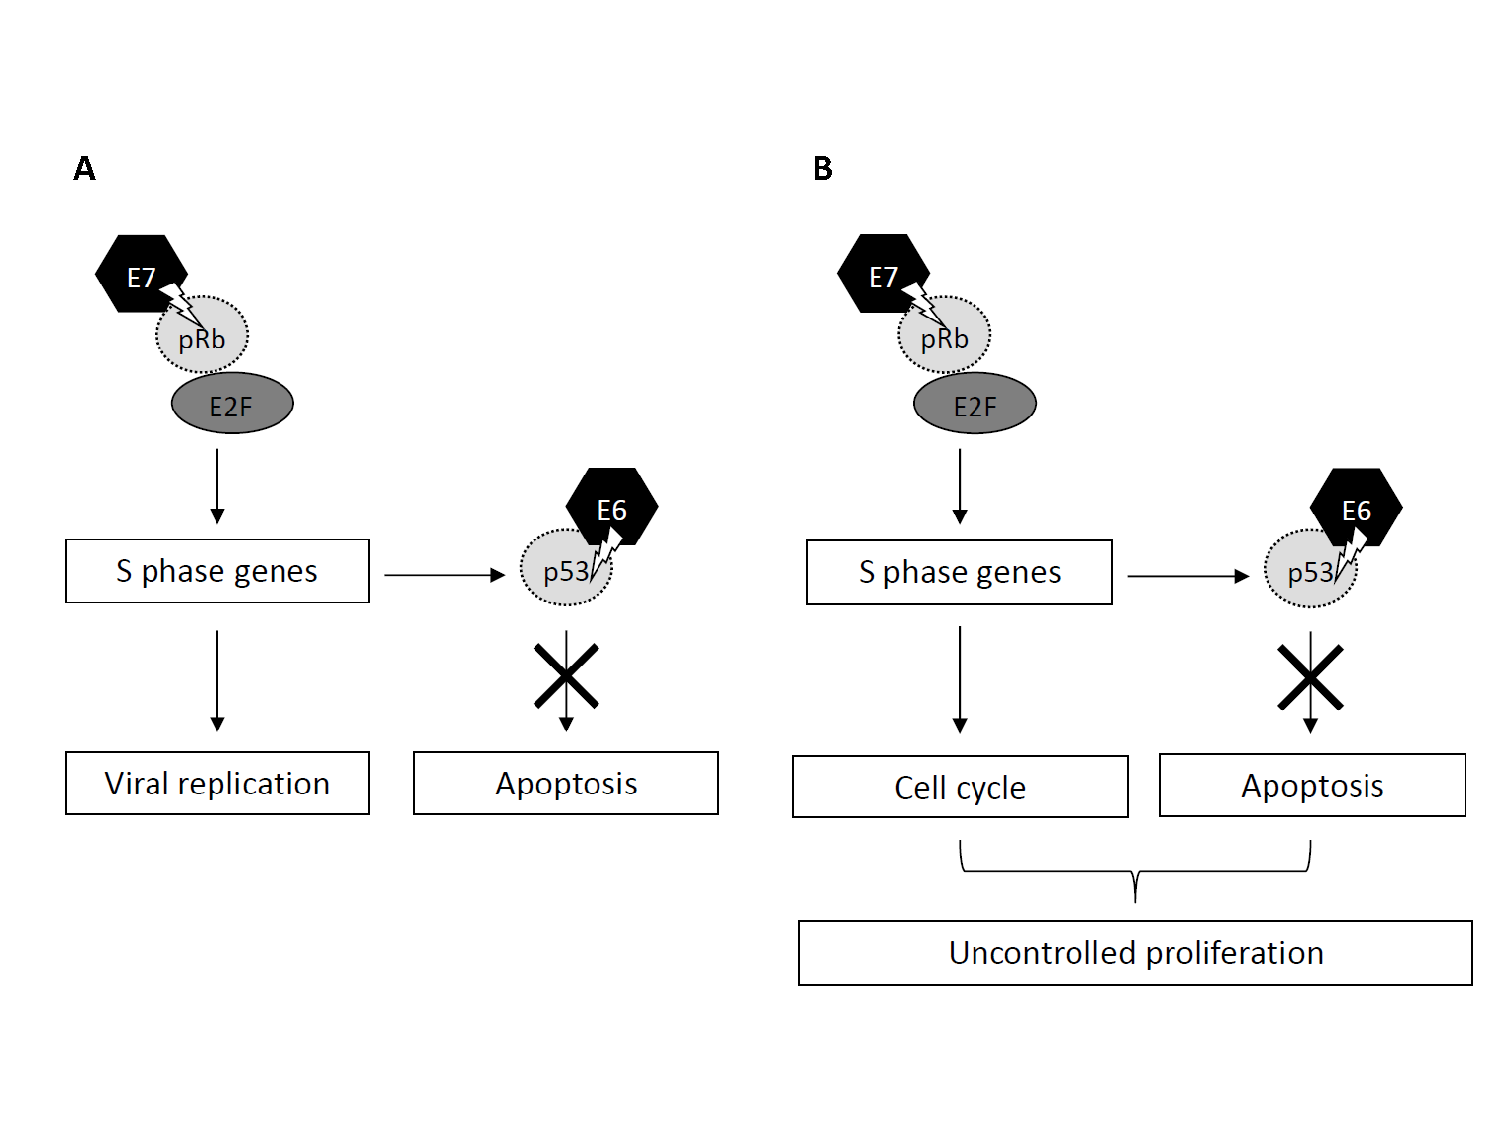
\includegraphics[scale=0.6]{viral2.pdf}\\
\end{tabular}
\caption{Effect of cellular events where E6 binds to p53 inducing its degradation, while E7 binds the Rb gene product and causes that transcription factor E2F becomes unbound and free to induce the viral replication in \textbf{A}. Later this lead to \textbf{B} where cell cycle activation together with appopthosis cause uncontrolled proliferation.}
\label{fig:viral}
\end{figure}

Viral oncogenes E6 and E7 are directly associated with chromosomal instability (reviewed in \cite{Wilting2016}). They encode proteins able to reactivate the cellular DNA replication machinery in non-dividing infected cells. Through direct and indirect interactions with cell cycle control and apoptosis mechanisms of the host cell, E6 and E7 can force non-dividing differentiating cells to start viral DNA replication, as illustrated in Figure $\ref{fig:viral}$. Aberrant expression of E6 and E7 in basal dividing cells of the epithelial layer results in uncontrolled cell cycling which in turn induces genetic instability. Viral oncogenes E6 and E7 are directly associated with chromosomal instability causing DNA damage, centrosome abnormalities and chromosomal segregation defects \cite{Duensing2004, Moody2010}. In addition, viral oncogenes were shown to increase the activity of enzymes responsible for DNA methylation. Hence, hypermethylation is a  frequent event during HPV-induced transformation.  The mechanisms behind aberrant E6 and E7 expression in dividing cells are still not completely elucidated. One potential mechanism involves integration of the viral genome in the genome of the infected cell, resulting in loss of regulation of the viral genes. However,  it remains unclear whether viral integration is a cause or consequence of chromosomal instability \cite{Pett2004}.

\subsubsection{Model system for HPV-induced transformation}

The development of cancer, as a genetic disease, is a complex and dynamic biological process. To better understand cervical cancer development and obtain more insight in the genes involved, we need to find ways to reduce the complexity of this process for analytical purposes. To address the complexity of cervical carcinogenesis we make use of a longitudinal in vitro system consisting of two cell lines immortalized with HPV16, and two with HPV18 (Figure $\ref{fig:experiment}$). In this model distinct stages of transformation can be recognized (extended lifespan, immortalization, and anchorage independence (reviewed in \cite{Steenbergen2005}) and this model was previously shown to faithfully mimic cervical precancerous lesions morphologically and (epi)genetically \cite{Steenbergen2004, Wilting2006, Henken2007}. All 4 cell lines originate from the same parental cells, which are transfected with HPV and cultured over time, thereby eliminating inter individual heterogeneity. During continuous culturing, cell lines become independent from each other, acquiring different modifications on the (epi)genetic level. 

\begin{figure}[h!]
\centering
\begin{tabular}{cc}
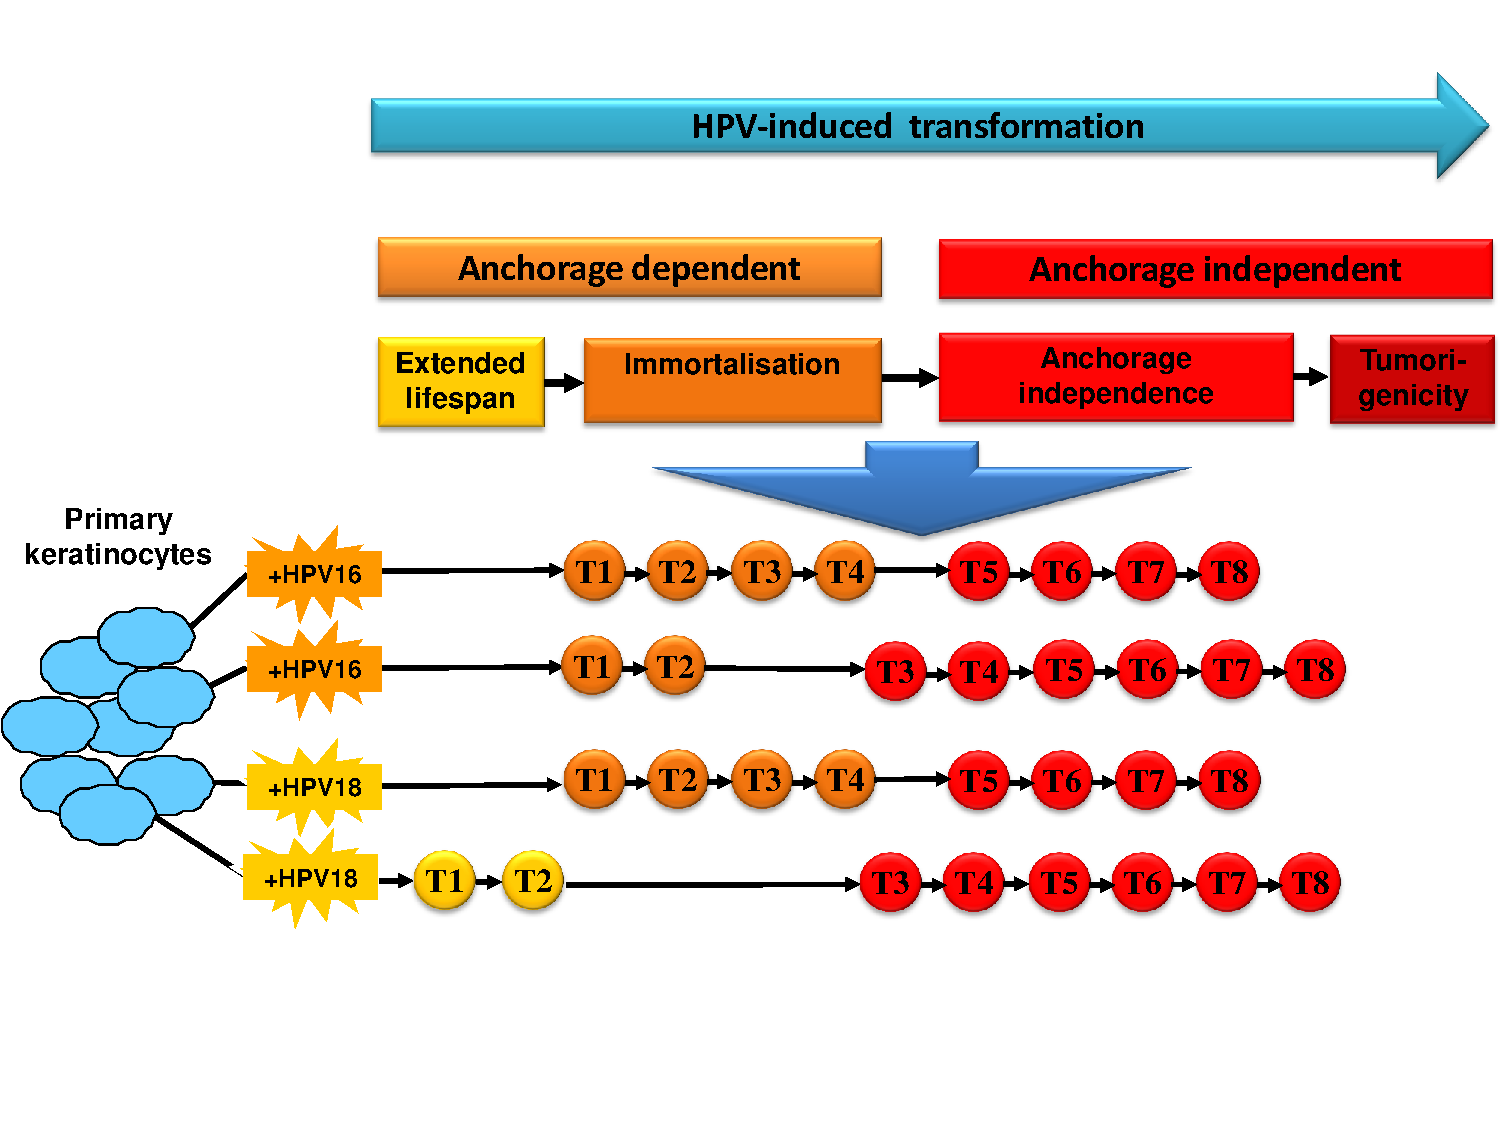
\includegraphics[scale=0.45]{experiment2.pdf}\\
\end{tabular}
\caption{The experimental layout. Colors indicate how time points are distributed over the stages of HPV-induced transformation.}
\label{fig:experiment}
\end{figure}

A major drawback to the use of cell lines in general is the absence of the micro-environment, including surrounding stromal– and immune cells and their secreted factors. However, there are also several advantages to the use of cell line models, including the availability of high-quality pure material and, as mentioned before, the elimination of inter-individual differences. Most importantly,  carcinogenesis in general is a dynamic biological process and our cell line model allows us to study the underlying kinetics over time.  In this way  we are able to model the order and temporal involvement of the identified alterations. 

\subsection{Data generation and analysis}

To obtain a comprehensive overview of the molecular alterations involved in HPV-induced transformation all four cell lines were assayed for DNA copy number and m(i)RNA expression at eight consecutive moments in time, which were distributed over the distinct stages of transformation, as is illustrated in Figure $\ref{fig:experiment}$. mRNA and miRNA expression levels were measured with and without demethylating treatment (5-aza-2'-deoxycytidine (DAC)). This treatment results in global DNA demethylation of the cells enabling us to indirectly measure DNA-methylation mediated silencing of genes during HPV-induced transformation on the transcriptome level.

Genome-wide high-throughput molecular profiling was performed using microarrays. The microarray technique appeared two decades ago \cite{Schena1995}, just after completion of sequencing of the whole human genome, and allowed for rapid developments in the field of biomedical research. This high-throughput technique allows for simultaneous measuring of thousands of predefined oligonucleotide sequences, representing either the human genome or transcriptome. Currently microarrays are being replaced by next generation sequencing, as a promising technique for measuring both the genome and transcriptome. This new sequencing technique offers several advantages compared to microarrays \cite{Wang2009}. It is not limited to known genomic sequences, allows for better quantification at the lower and upper (no limit) end of the spectrum, and shows less experimental noise. Although sequencing provides several advantages over microarrays, the latter still represents a widely used and easy-to-use laboratory method for which various validated data analysis pipelines and interpretation tools are available. For the purpose of our study both techniques were suitable. As we had more experience with microarray data analysis we chose that method, however, in principle, all tools developed in this project can be extended to deal with sequencing data as well as illustrated in Chapter 2 \cite{Miok2014} and further discussed in Chapter 7 (Discussion). Distinct levels can be recognized in the analysis of genomic and transcriptomic time series : 1) Experimental design, 2) Preprocessing, and 3) Statistical analysis. These steps will be discussed below. 

\subsubsection{Experimental design}

To accurately and precisely measure the effect of interest using microarrays in our cell line model, we need to have a proper design of the experiment. Measuring in parallel such a large number of biological sequences, has consequences for the design of the experiment. A proper design makes sure that questions of interest can be answered, under the given conditions. Additionally, to have informative results, we need to be able to separate uncontrolled variation (noise) in the microarray experiment from actual differences between the conditions. In our experiments this is achieved by applying the principles of microarray design: blocking, balancing and randomization of the samples. All these techniques are essential to get trustworthy results.


\begin{figure}[h!]
\centering
\begin{tabular}{cc}
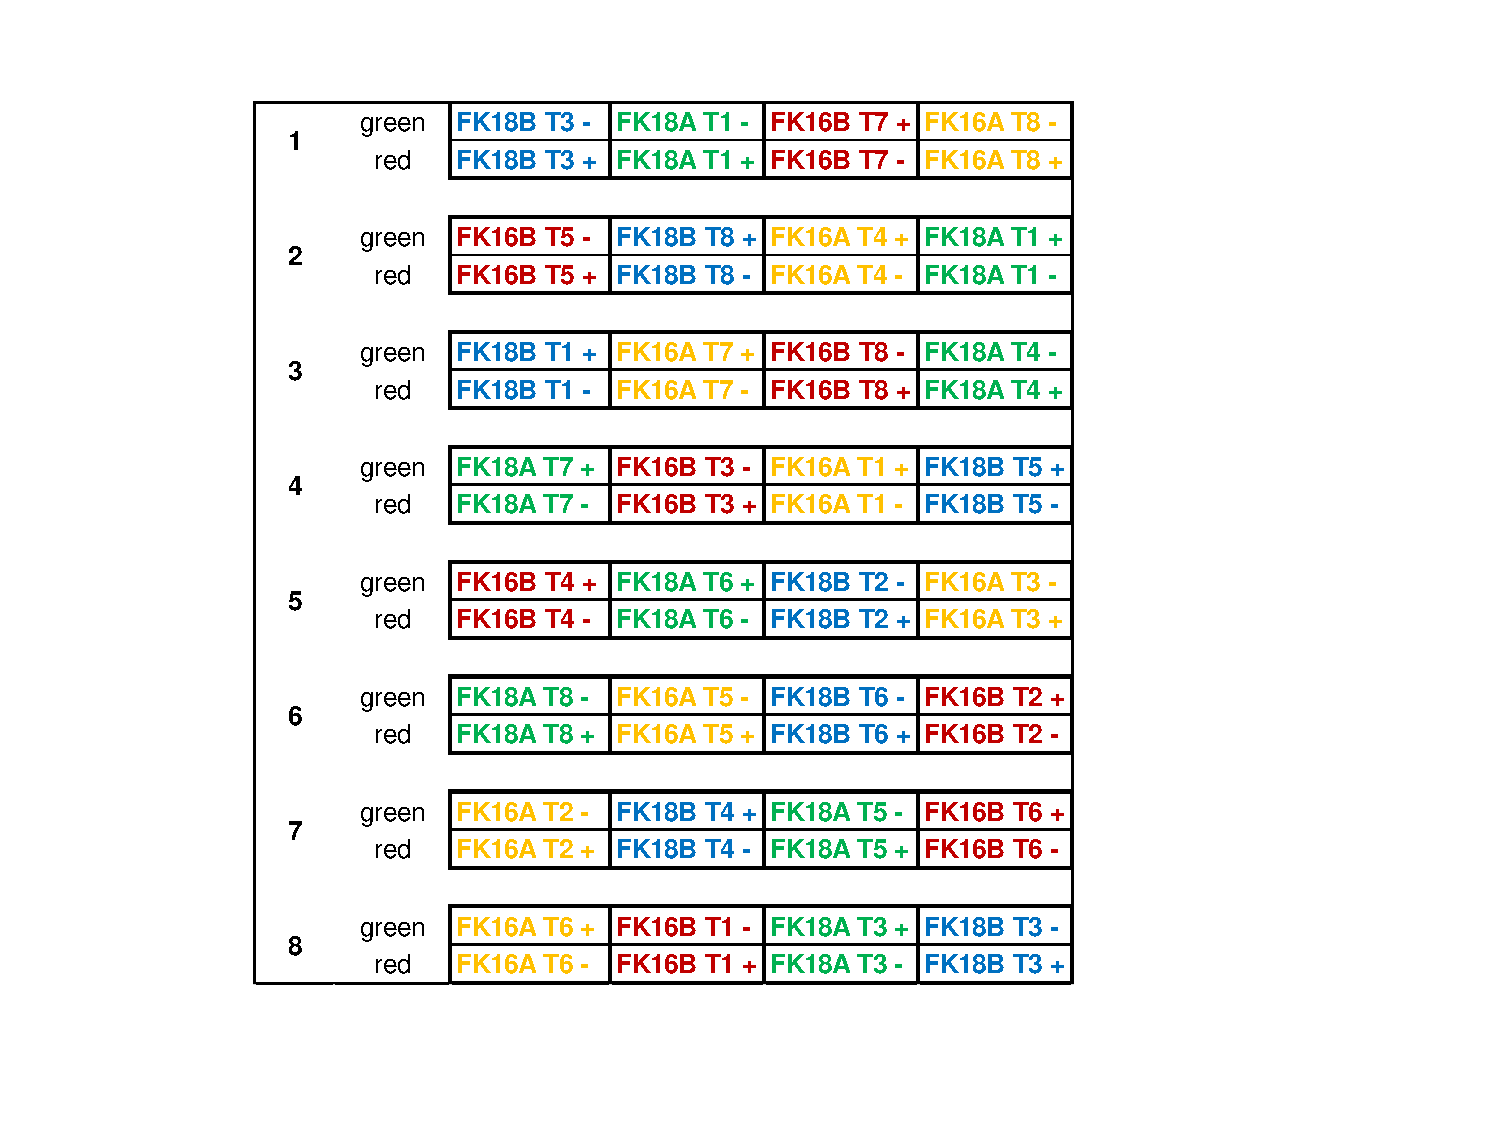
\includegraphics[scale=0.53]{mRNAdesign.pdf}
\end{tabular}
\caption{Illustration of the 8 slides from the double-channel (green and red) mRNA gene expression experimental design. Name of the sample indicates cell line (FK16A, FK16B, FK18A and FK18B), time point (T1 to T8) and treatment (DAC + treated and - untreated samples). For better illustration all cell lines are represented by different colors.}
\label{fig:experimentDesign1}
\end{figure}

\begin{figure}[h!]
\centering
\begin{tabular}{cc}
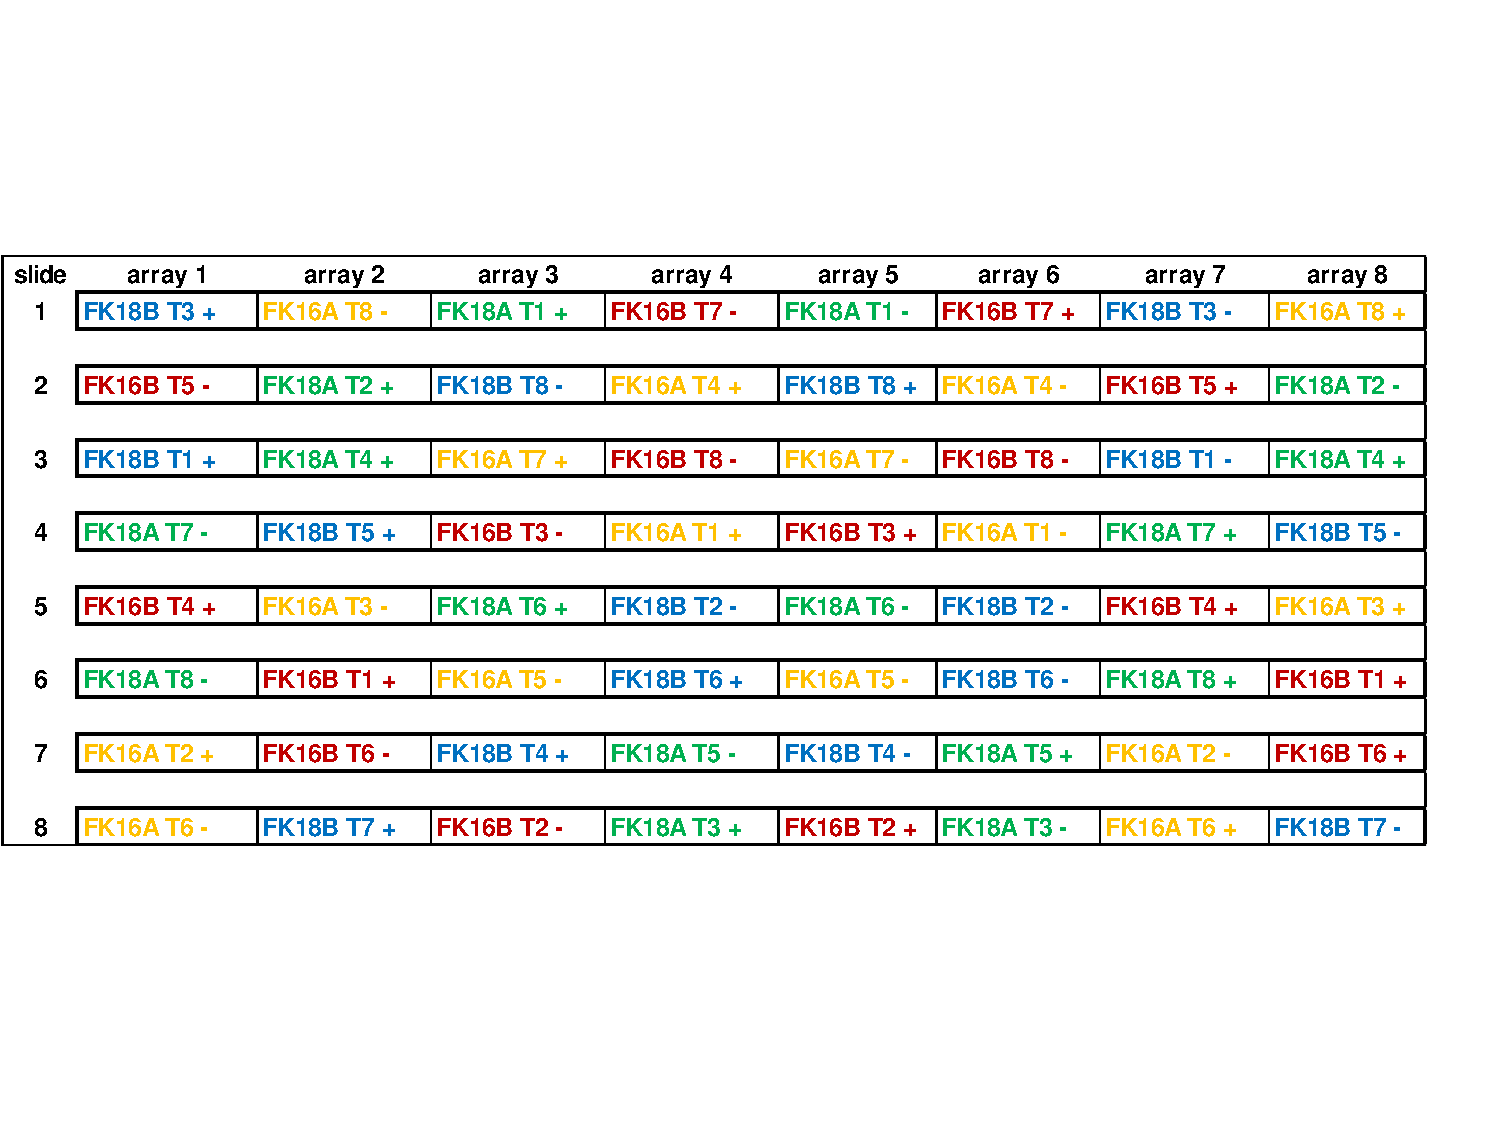
\includegraphics[scale=0.49]{miRNAdesign.pdf}
\end{tabular}
\caption{Illustration of the 8 slides from the single-channel miRNA gene expression experimental design. Name of the sample indicates cell line(FK16A, FK16B, FK18A and FK18B), time point (T1 to T8) and treatment (DAC + treated and - untreated samples). For better illustration all cell lines are represented by different colors.}
\label{fig:experimentDesign2}
\end{figure}

\begin{itemize}
\item \textbf{Blocking:} In the micorarray experiment undesirable variability between conditions are higher among slides, while it is presumed to be (more) homogeneous within slides. The blocking principle suggests to form a homogeneous set of experimental runs, called blocks, to protect against this foreseeable source of variability. Within a two-sample study blocking assigns samples from both conditions (i.e. treated and untreated) to the same block. This ensures that the group effect can be disentangled from the slide effect, as the group effect can be estimated from the `within-slide contrast'.

\item \textbf{Randomization:} Microarray hybridizations are carried out sequentially. During this period experimental conditions may change. For instance, due to changing weather conditions affecting the chemistry. Suppose we would deal with a two-sample study in which we hybridized all samples of one condition first followed by those of the other condition, any effect due to the treatment would be confounded with time. The order in which hybridizations are carried out is randomized. In such a randomized experiment an estimate of the group effect is no longer associated with time. Moreover, randomization ensures the validity of the statistical inference in the analysis of the experiment.

\item \textbf{Balancing:} Balancing ensures that the comparison of interest is not confounded with the position on the slide. It requires that each factor setting is represented equally within each block: each position has an equal number of replicates of all levels. This ensures contrasts/effects can be estimated optimally.
\end{itemize}
 
For DNA copy number we did not need to apply blocking, randomization and balancing as DNA was previously found to be sufficiently stable under varying experimental conditions \cite{Buffart2008}. As we used dual-channel arrays, we made sure that on every slide a reference sample was present in both channels. In addition, reference samples were obtained from the parental cells from which the cell lines were derived. Using the parental cells as a reference eliminates the detection of DNA copy number variation between two normal individuals.

For mRNA (double channel) and miRNA (single channel) expression analysis we did apply blocking, randomization and balancing (Figure $\ref{fig:experimentDesign1}$ and Figure $\ref{fig:experimentDesign2}$). One slide contains either 4 dual channel arrays (mRNA) or 8 single channel arrays (miRNAs). Each slide included material from all 4 cell lines (randomization), both treated and untreated samples were hybridized together in one array (block), and time points and positions on the slide were balanced. As the platform used for mRNA detection was a dual-channel platform, conditions, time points and cell lines were also blocked, randomized and balanced over the two channels. 

\subsubsection{Data preprocessing}

After performing the microarray experiment, following the above described experimental design, raw data were generated. A very important first step in the analysis of the data from microarrays is preprocessing. Data generated from the microarray experiment comprise true biological signal and experimental artifacts. The experimental or technical artifacts are induced by systematic and experimental variation, while true biological signal consists of "wanted" variation among cell lines and time points. Hence, preprocessing aims to remove experimental artifacts to make different samples comparable. The main steps discerned in preprocessing of microarray data are 1) background correction, 2) normalization and, for DNA copy number analysis, 3) segmentation, which are explained in detail below.

\begin{itemize}  
\item \textbf{Background correction:} Intensities obtained as the result of measuring samples using oligonucleotide microarrays comprise foreground and background signal. The initial step in preprocessing of gene expression data is transformation of the intensities into quantities without background signal. The foreground measurement contains the true biological signal. On the other hand, background intensities may be influenced by unspecific sources, such as auto-fluorescence of the array surface, non-specific binding, printing errors, scratches, and dust particles. Hence, background correction methods intend to estimate and remove signal induced by these sources.

\item \textbf{Normalization:} Normalization intends to remove experimentally induced variation. Normalization makes $\log_2$ ratios of different hybridizations comparable by reducing experimental bias between (hybridizations) and within (red and green fluorescent signals) arrays. Removal of experimental artifacts while preserving the true biological signal has significant impact on the identification of differently expressed genes.

\item \textbf{Segmentation (only for DNA copy number analysis):} The segmentation algorithm divides the genome into non-overlapping segments with equal DNA copy numbers. Segments are separated by break points. Break points represent locations between two adjacent segments with different relative DNA copy number. Modeling of the DNA copy number with segment lines reduces the noise, improves detection of aberrations and makes the identification of break points more obvious see \cite{Wiel2011}.
\end{itemize}
 

\paragraph{DNA copy number data:}

The first preprocessing step of DNA copy number data is normalization. Ratios of samples from cell lines and reference were subjected to median normalization \cite{Wiel2007}. After applying median normalization data are centered such that the median value becomes zero. A profile of one normalized sample is illustrated in left panel of Figure \ref{fig:CGHnormalization}. The next step in the preprocessing of DNA copy number data is segmentation. Procedures include circular binary segmentation (CBS) algorithm \cite{Olshen2004}. Figure \ref{fig:CGHnormalization} shows an example of a segmented profile, where part of the probes were removed in order to highlight the segmentation line.

\begin{figure}[h!]
\centering
\begin{tabular}{cc}
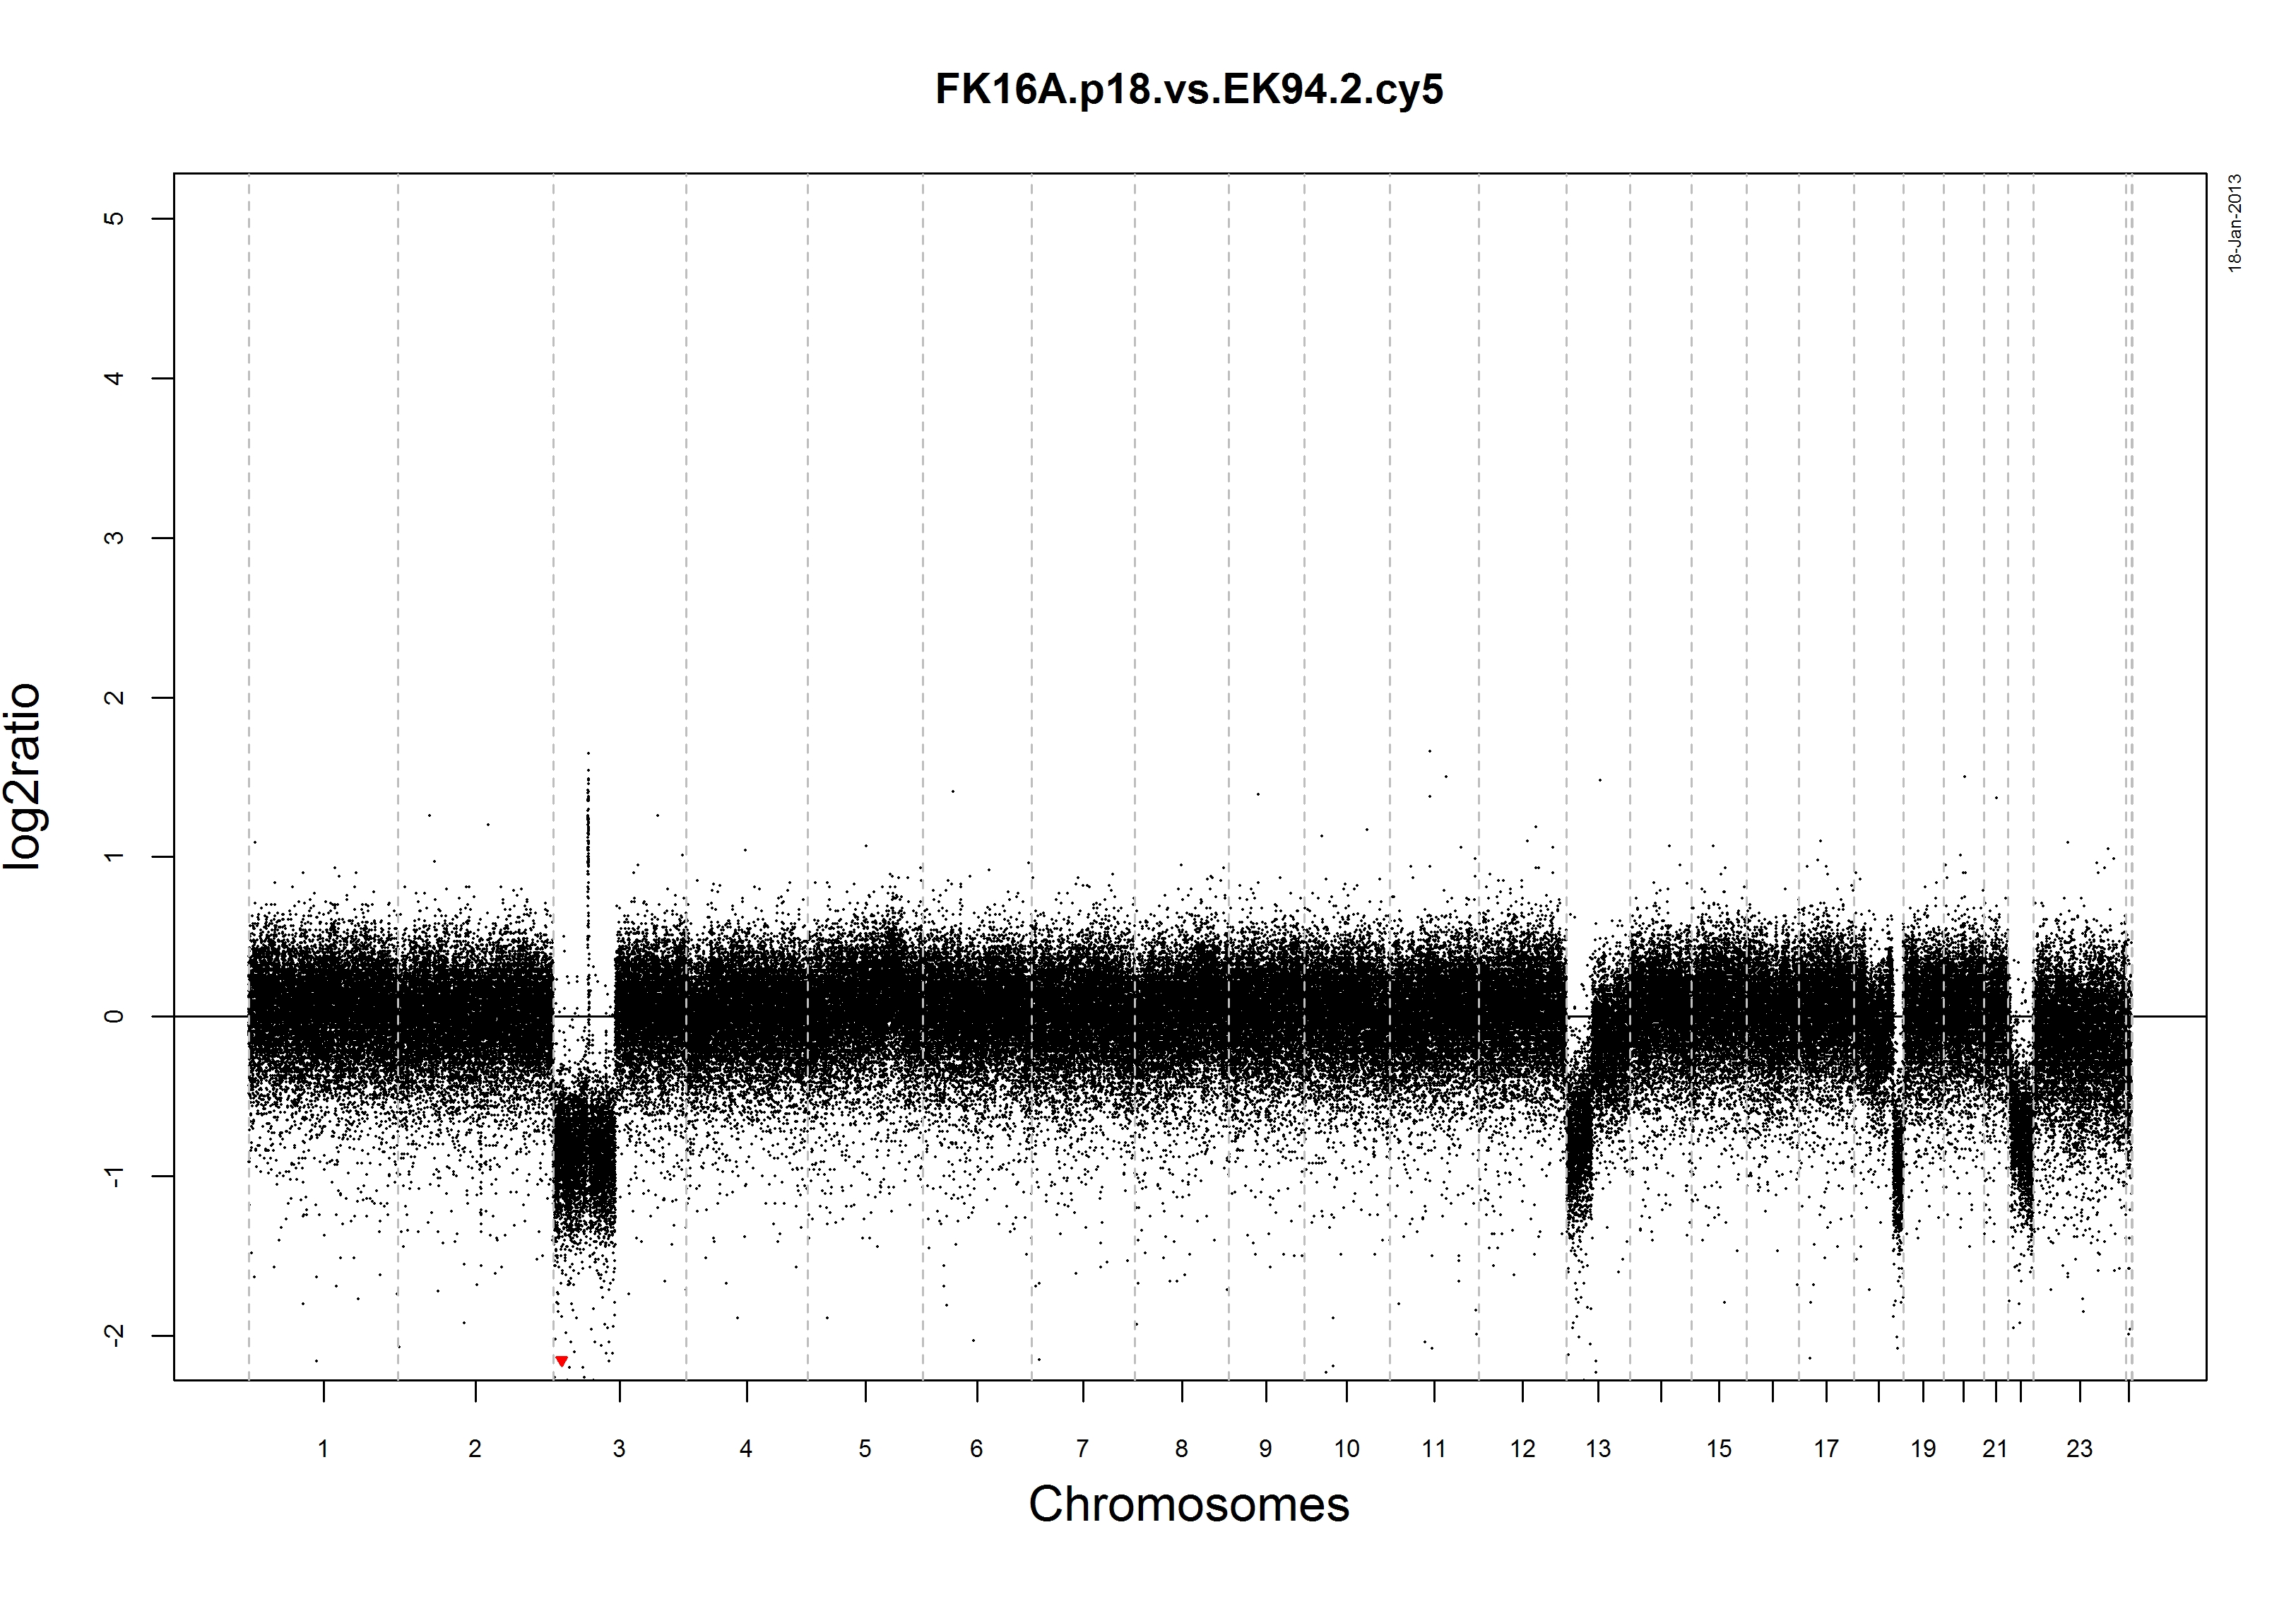
\includegraphics[scale=0.35]{noWavesCorrected.jpeg}\\
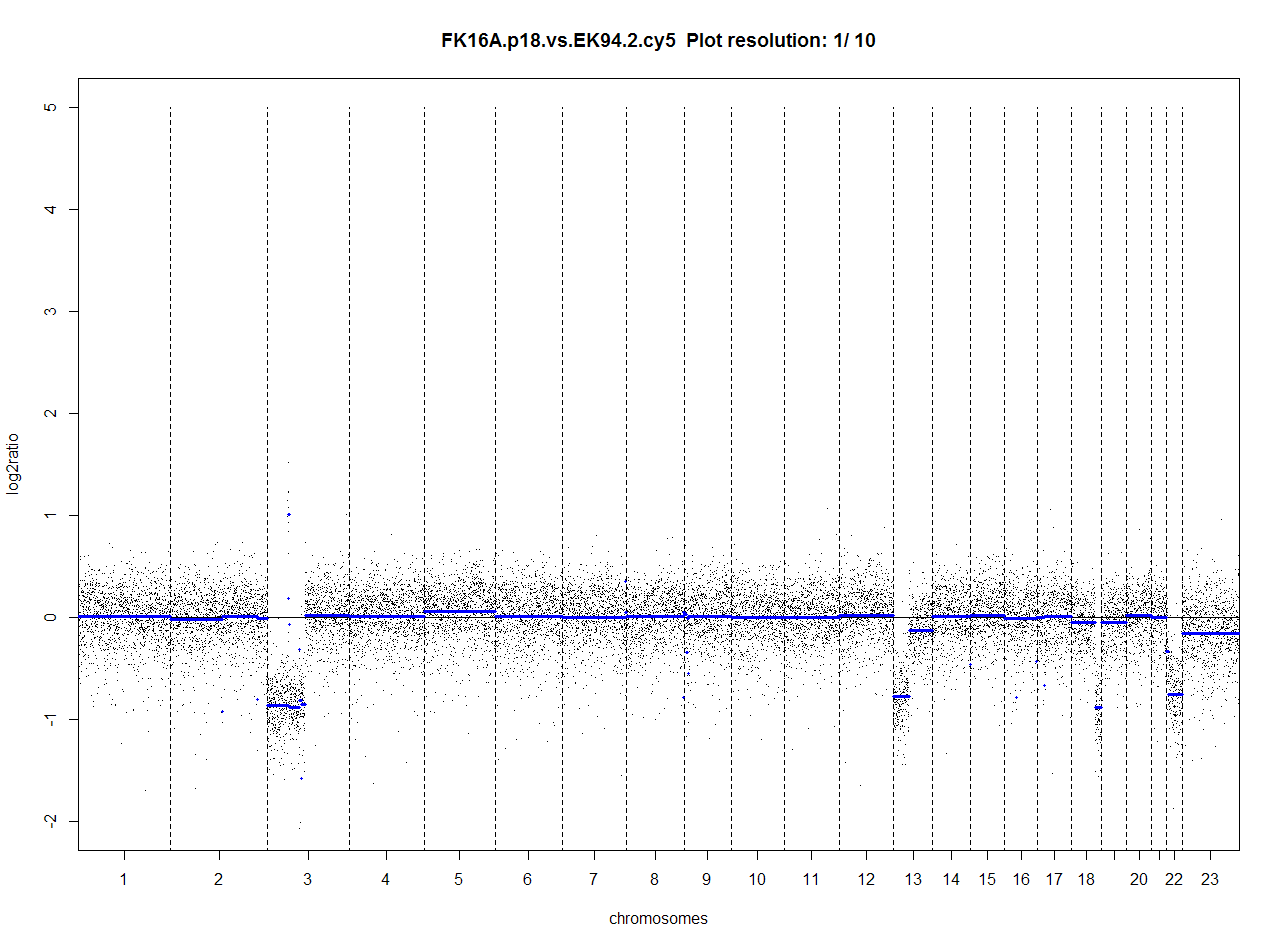
\includegraphics[scale=0.21]{CGH_preproc2.jpeg}  
\end{tabular}
\caption{DNA copy number profile of one sample. The left panel represents the profile after normalization, while the right panel after segmentation.}
\label{fig:CGHnormalization}
\end{figure}

\paragraph{mRNA gene expression data:}

 The preprocessing of mRNA gene expression data comprised background correction and normalization. Background correction was performed using the R package ${\tt limma}$, the RMA method based on convolution model described in \cite{Ritchie2007, Silver2008}. As the demethylating treatment is expected to result in overall higher gene expression values we need to take treatment into consideration while normalizing the data. Hence, normalization is applied separately for treated and untreated samples. Normalization of the samples between arrays was performed using a robust quantile method, which incorporates calibration using weighted quantile normalization employing Huber's psi function and variance stabilization via $\log_2$ transformation. Figure \ref{fig:mRNAnormalization} illustrates the density plot of the sample intensities before normalization. There are clusters of samples with higher intensities probably due to technical variation. After applying normalization density plots in Figure \ref{fig:mRNAnormalization} indicated that samples are comparable, enabling us to continue with  further analyses.  

\begin{figure}[h!]
\centering
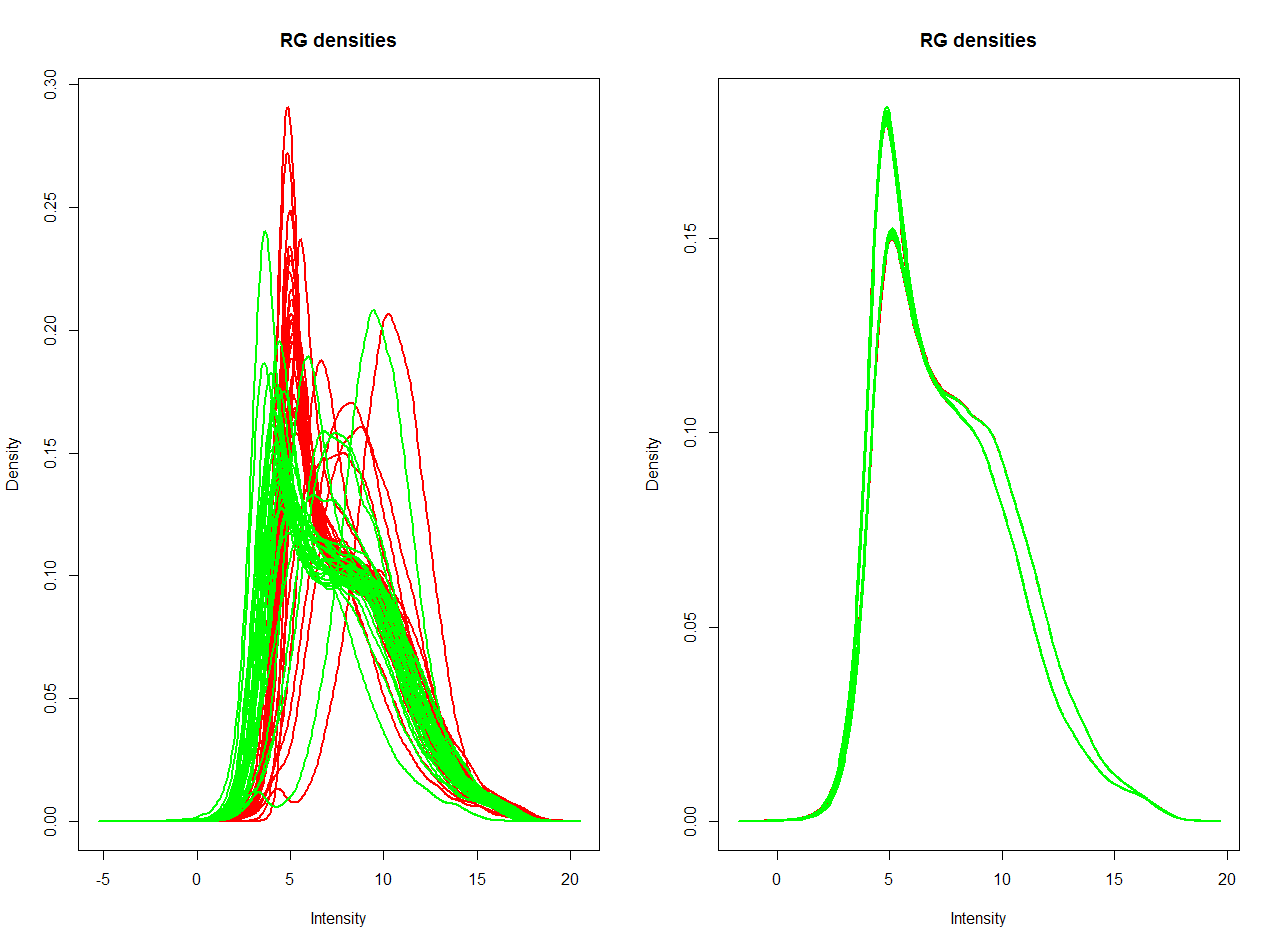
\includegraphics[scale=0.3]{mRNA-DensityPlot.jpeg}  
\caption{Density plot of the intensities, where each line represents one sample. The left panel illustrates arrays before normalization, while the right panel represents the arrays after the normalization.}
\label{fig:mRNAnormalization}
\end{figure}

\paragraph{miRNA gene expression data:}

\begin{figure}[h!]
\centering
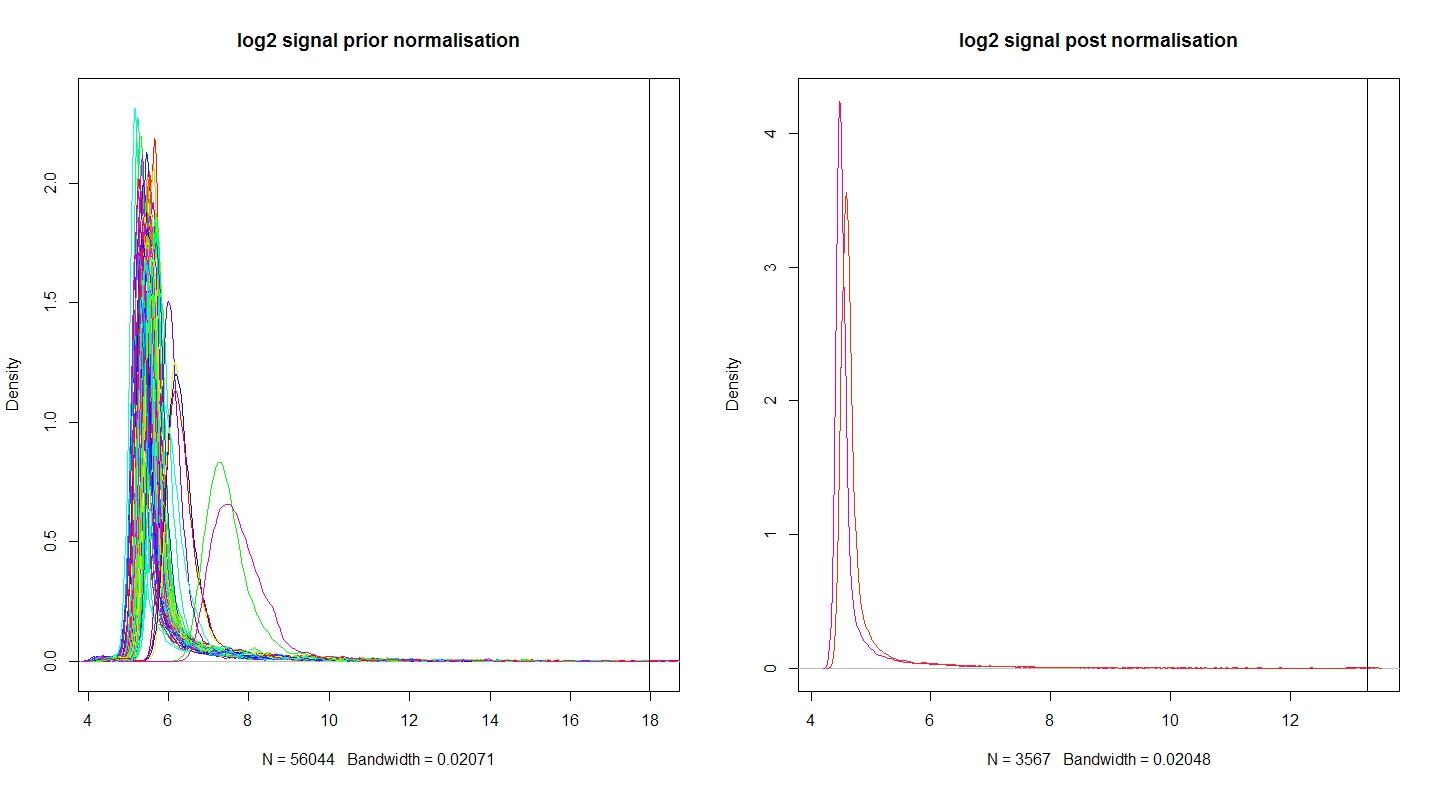
\includegraphics[scale=0.3]{Before-AfterNormalization.jpeg}  
\caption{The left panel illustrates a density plot of the miRNA arrays before normalization, where each line represents one sample. The right panel represent the arrays after normalization.}
\label{fig:miRNAnormalization}
\end{figure}

Preprocessing of miRNA gene expression data essentially follows the same steps as for mRNA gene expression data. Due to a different labeling strategy where only one fluorophore is incorporated per miRNA molecule, intensities before preprocessing were quite low. Because the distribution of background intensities among the samples was uniform, subtracting background signal could obstruct identification of differential gene expression by production of negative expression values. Therefore, this step in preprocessing was omitted. In Figure \ref{fig:miRNAnormalization} density plots of the miRNA samples are illustrated before and after normalization. To facilitate downstream analyses, replicates of the same probe were averaged.

\paragraph{DNA methylation data:}
 Preprocessing of DNA methylation data was performed applying a pipeline for Infinium HumanMethylation450K BeadChip data proposed by \cite{Touleimat2012}. This preprocessing pipeline takes the different chemistry underlying type I and type II probes present on this platform into account by employing a subset  quantile normalization approach. The method returns normalized Beta values that are representative of the percentage of methylation for that particular CpG dinucleotide.


\subsection{Statistical analysis}

To gain more insight into the sequential order of molecular events necessary for cervical carcinogenesis we performed a longitudinal, multi-level molecular characterization of HPV-transformed cell lines. 
However to analyze the obtained data in an integrative manner, novel statistical methodology is required. Over the years many statistical methods for analysis of time-course omics data have been proposed. They often focus on a single molecular level. Moreover, many lack a clear functionally motivated statistical model. Hence, we developed temporal integrative statistical methodology for multilevel time-course molecular data. The statistical methodology developed here can be applied to the multilevel time-course molecular datasets of other cancer types and model systems. 

The methodology presented in this thesis analyses the data with respect to two different statistical units of interest: the unit of a single gene and the unit of a group of genes that shares a known biological function, called pathways. Univariate statistical methodology is developed to perform integrative temporal differential gene expression analysis of the single gene unit. On the other hand, pathways are groups of genes from different genomic locations, which work together. Pathway analysis requires development of novel multivariate methodology to identify temporal and contemporaneous interactions among genes.

\subsubsection{Differential expression analysis}

Knowledge of differentially expressed genes may improve our understanding of the molecular basis underlying the mechanism of carcinogenesis. The problem of identifying differentially expressed genes is commonly addressed, both from the static and temporal perspective. The static view-point focuses on identifying differentially expressed genes between two conditions, while the temporal viewpoint studies the changes in the gene expression over time. Due to the fact that the regulation of gene expression is a dynamic process it is more appropriate to address this problem from the temporal perspective.

Many statistical models have been developed to address the problem of temporal differential expression analysis from microarray experiments. The first method \cite{Nau2002, Shapira2009} used ad-hoc approaches to select genes as differentially expressed based on the criterion that at least two consecutive time points are above a chosen fold change. This approach uses an arbitrary threshold dependent on the baseline expression levels, which may not be appropriate for all genes. Methods like $\texttt{SAM}$ \cite{Tusher2001} try to overcome this problem employing modified version of t-test. Another popular method is $\texttt{LIMMA}$ \cite{Smyth2004} which uses an empirical Bayes estimate of the variance for each gene, while the differential expression analysis is performed using a classical t-test, through dividing the time domain into two groups. All these methods are not applicable given the design of our experiment.

A range of more sophisticated statistical methods were developed over the years, which can be divided in three groups. Several of these methods extend the empirical Bayes framework to time series analysis \cite{Efron2001, Lonnstedt2002, Eckel2004, Tai2006}. Alternative approaches proposed by \cite{BarJoseph2003, Storey2005, Hong2006} involve univariate spline-based methods, which fit a smoothed curve to the longitudinal data and detect differential expression employing a statistical test. Finally, $\texttt{BATS}$ combines these two approaches. It employs gene-wise functional modeling to explain temporal differential gene expression, which is implemented in a hierarchical Bayesian framework. All these methods perform temporal differential expression analysis taking into account only a single (mRNA gene expression) molecular level. Integration of omics data may enhance the investigation of the genomic mechanisms involved in carcinogenesis.

Integrating multilevel molecular data may significantly improve temporal differential expression analysis, allowing for an effective way to pool the information across multiple datasets. For example DNA copy number is linked to mRNA expression levels. This relationship can be incorporated in differential gene expression analysis, identifying genes with significant variation in expression levels associated with copy number changes. These genes represent potential tumor suppressor genes and oncogenes involved in the carcinogenic process. Hence, we developed a method which relates these two molecular levels over time. The method estimates the amount of the variation in expression levels induced by copy number abnormalities over time, selecting better candidates through significance analysis.

\subsubsection{Analysis of the dynamics within the pathway}

Currently in the literature the understanding of cancer complexity is moving from the gene level to pathways. This results in increasing interest in the reconstruction of gene regulatory networks. Over the years various methods were developed for dynamical gene regulatory network reconstruction. The methods of \cite{Song2009} ($\texttt{TV-DBN}$), \cite{Lebre2009} ($\texttt{G1DBN}$), \cite{Rau2010} ($\texttt{EBDNB}$) model the data by a dynamic Bayesian network. Other methods use mutual information as a measure of dependencies between two genes at different time delays \cite{Zoppoli2010} ($\texttt{TimeDelay-ARACNE}$), \cite{Meyer2007} ($\texttt{MRNET}$), \cite{Faith2007} ($\texttt{CLR}$)). The latter methods are computational approaches, lacking a solid statistical model. Alternative approaches involve vector autoregressive models, which aim to capture linear interdependencies among gene expression levels in order to reconstruct time-series chain graph (\cite{Charbonnier2010} ($\texttt{simone}$), \cite{Abegaz2013} ($\texttt{SparseTSCGM}$)). The method proposed by \cite{Charbonnier2010} reconstructs a regulatory network parametrized only by autoregressive model parameters and the innovations (errors) are assumed independent. On the other hand, \cite{Abegaz2013} addressed the problem of the full likelihood of the first-order vector autoregressive model, estimating both temporal and contemporaneous interactions. Lasso regularized regression performs estimation and models selection simultaneously, allowing a sparse solution. Such an approach is not always an advantage, especially when more accurate representations of the parameters are required \cite{Wieringen2016}. Parameter estimation followed by support determination may allow better performance with respect to the inclusion/exclusion of edges. Moreover, it may better determine individual partial correlation or precision estimates after sparsification.

In this thesis, high-dimensional data from time-course experiments are modeled using vector autoregressive process, where the model parameters are estimated through ridge penalized likelihood maximization. Imposing ridge penalties results in non-sparse autoregressive and precision model parameter estimates. To determine edges of main interest post-estimation significance analysis is employed (\cite{Efron2004, Strimmer2008}). Estimation may be improved by incorporating prior knowledge on both autoregressive and precision parameters in order to obtain less biased estimates. In the Chapter 4 the methodology is further extended to answer related biological questions. One of the extensions comprises multilevel molecular integration analysis which allows to reconstruct pathways from DNA copy number, mRNA and miRNA gene expression data. Another may be the identification of differences in the dynamics of particular molecular pathways between distinct groups/classes of longitudinal samples (e.g. cell lines affected with HPV16 and HPV18).

Finally, the presented methodology is employed to obtain a dynamic view of the (epi)genetic changes of measured HPV-transformed keratinocyte cell lines (see Chapter 5). To capture the temporal variation in the m(i)RNA gene expression is related univariately to the DNA copy number changes using the methodology presented in Chapter 2.  This analysis identified around 33$\%$ of m(i)RNAs to be differentially expressed over time, partially attributable to abnormalities in DNA copy number. The same methodology is used to model the association between miRNA and mRNA over time in order
to identify miRNA targets. Based on enrichment analysis three well-known pathways are identified to be enriched within the set of genes that exhibited DNA copy number related differential expression. These three pathways are further scrutinized by the multivariate analysis of Chapter 3 to obtain a 
picture of the dynamics within the pathways. This yielded putative regulators and regulatees for each
pathway. These genes may provide novel biomarkers for early detection of cervical
cancer as well as potential therapeutic targets.


\newpage
\subsection{Outline of this thesis}

The thesis is divided in six chapters, which are briefly summarized here.
\\
\\
\textbf{Chapter 2:} \textit{ {\tt{tigaR}}: integrative significance analysis of temporal differential gene expression induced by genomic abnormalities}

In this chapter we propose the methodology to improve temporal differential gene expression in terms of the sensitivity, specificity and reproducibility, as well as to allow more relevant biological questions to be addressed. Our method is extended to incorporate concordant relationship between DNA copy number and gene expression molecular levels. Hence, the method allows us to identify not only consistently altered genes over time, but also to assess whether this is caused by DNA copy number abnormalities. Spatial structure is taken into account inducing dependency between genomic neighboring features. Estimation of the model parameters is performed using an empirical Bayes. This allows us to borrow information over the genes and from neighboring features, resulting in more stable estimates. All this allows us to have a broader overview of abnormalities at multiple molecular levels, as well as to have a better selection of potentially interesting genes. By modifying the link function our method can handle count RNA-seq data as well. Illustration of the methodology is performed on HPV-induced transformation (microarray) and head $\&$ neck cancer (RNA-seq) data. 
\\
\\
\textbf{Chapter 3:} \textit{Ridge estimation of the VAR(1) model and its time series chain graph from multivariate time-course omics data}

Chapter 3 studies network reconstruction of both temporal and contemporaneous interactions among genes using the first-order vector auto-regressive (VAR(1)) process. It is argued that employing regularization based on ridge penalization is better or at least equally good as popular approaches \cite{Abegaz2013} using lasso penalty. Methodology allows to incorporate prior knowledge on non-existent interactions among the genes providing less biased estimates of the temporal and contemporaneous interactions among the genes. Several down-stream analyses for exploiting the reconstructed time-series chain graph are presented: node statistics, impulse response analysis, mutual information analysis, path decomposition and motifs illustration. Finally, we illustrate our method on the data from the aforementioned HPV-induced transformation experiment mapped to the p53 signaling pathway, known to be altered due to HPV E6-induced p53 degradation (from KEGG repository). 
\\
\\
\textbf{Chapter 4:} \textit{Ridge estimation of network models from time-course omics data}

In this chapter methodology proposed in the Chapter 3 is extended in several directions, to address further biological questions, employing more complex vector autoregressive models. First, a VAR(2) model is considered, where we use an additional time point to explain the current one. Second, in order to reconstruct regulatory networks of multilevel molecular data, VAR(1) model is extended with time-varying covariates, eg. DNA copy number and miRNA gene expression data. Finally, regulatory networks can differ in distinct sample groups (i.e. HPV16 versus HPV18). This can be identified assuming a VAR(1) model per group of samples augmented, with fused ridge penalty. Methodology from both Chapter 3 and Chapter 4 is implemented in R-package ${\tt ragt2ridges}$ freely available from CRAN. We present detailed illustration of the package on the data from the cell line experiment mapped to the p53 signaling pathway (from KEGG repository).
\\
\\
\textbf{Chapter 5:} \textit{Comprehensive molecular profiling of HPV-induced transformation over time}

To obtain a longitudinal overview of (epi)genetic alterations and resulting changes in gene expression involved in HPV-induced transformation, we obtained chromosomal, mRNA and miRNA expression profiles  at 8 different time points in 4 individual HPV-transformed keratinocyte cell lines arising from the same parental cells. Interestingly, unsupervised hierarchical clustering highlighted the role of chromosomal alterations in the acquisition of anchorage independence. 
{\tt tigaR} analysis (Chapter 2) revealed that around 1/3rd of differentially expressed m(i)RNAs over time is directly related to DNA copy number changes. Subsequent pathway analysis showed that focal adhesion (KEGG hsa04510), TGF-beta signalling (KEGG hsa04350), and mTOR signalling (KEGG hsa04150) were enriched within these copy number related differentially expressed genes. Employing the methodology described in the Chapter 4, ID1 and PITX2 were identified as main regulators of the altered TGF-beta signalling pathway, BRWD3 and NF2 for mTOR signaling, while PIGT and DAPP1 for focal adhesion pathway. In addition, we showed that {\tt tigaR}s can also be used to identify miRNA targets by modelling miRNA-mRNA interactions over time. The validity of this approach is shown by functional validation experiments.
\\
\\
\textbf{Chapter 6:} \textit{Aberrant methylation-mediated silencing of microRNAs contributes to HPV-induced anchorage independence}

 In this chapter we set out to investigate the contribution of methylation to miRNA expression changes related to the acquisition of anchorage independence. Methodology developed in Chapter 2 was not used as we noticed that effects of the demethylating treatment were substantially varying per cell line and per time point. Therefore, the ranking analysis was employed instead on the delta values between treated and untreated cells per time point and cell lines and integrated these results with results from the Illumina 450K Infinium methylation assay. Using this pipeline we identified hsa-mir-129-2/-137/-935/-3663/-3665 and -4281 miRNAs potentially silenced by methylation, for which we could validate hsa-mir-129-2/-137/-3663 and -3665. Interestingly, mature miRNAs derived from epigenetically silenced genomic locations were found to alter cell viability and the ability of cells to grow anchorage independently. This further supports the validity of our model system and indicates that molecular changes identified over time in these cells represent functionally relevant events.
